\section{PRELIMINARIES}
\label{sec:pre}
In this section, we introduce some basics about watermarking techniques, features of vector map like digital road map.


\subsection{Watermarking Techniques}

Every vector map has a precision tolerance which gives the maximum amplitude of the allowed
distortions for coordinates. The distortions of coordinates definitely below the tolerance
will not degrade the map's validity. 

\subsubsection{Data Usability Measurement Metrics}

Usability measurement metrics define the usability of a dataset. \cite{DBLP:conf/itcc/Sion02} 
gives a formal definition of usability measurement metrics and presents an allowable 
distortion bounds for a given input data. Different applications require different usability metrics. 
In numerics datasets including digital road maps,$a$ $mximum$ $allowable$ $mean$ $quare$ $error$ 
is widely used as the usability metric. Given an original dataset S and a watermarked dataset V,
${s}_{i}\in S$ and ${v}_{i}\in V$, the usability metric is defined in terms of mean squared error 
tolerances as follows:

${({s}_{i}-{v}_{i})}^{2}<{t}_{i},\forall i=1,...n$

$\sum {{({s}_{i}-{v}_{i})}^{2}<{T}_{max}}$

where ${t}_{i}\in T$, and it gives the error bound of watermarking. 
Similarly, assume the attacked dataset is W and ${w}_{i}\in W$. We can define the
$maximum$ $allowable$ $mean$ $square$ $error$ by attacks as follows:

${({s}_{i}-{v}_{i})}^{2}<{l}_{i},\forall i=1,...n$

$\sum{{({s}_{i}-{v}_{i})}^{2}<{T}_{max}}$

where ${l}_{i}\in L$ and $\sum {{{t}_{i}}^{2}}\gg {t}_{max}$

and it gives the error bound of attacks. 
${({s}_{i}-{v}_{i})}^{2}<{l}_{i}$ means that just several
least significant bits, ${m}_{1}$ LSBs, can be changed.
$\sum{{{t}_{i}}^{2}}\gg {t}_{max}$
 means the sum of changes for all individual data
items will be much more greater than the overall change in
the dataset. This is the basic requirement for all numeric
datasets. Otherwise, attackers just need to change values of
all data items to their allowable errors and beat any water-
marking technique.



\subsubsection{Attacks on Watermarks}
As explained in last subsection, if attackers want to change
all data items, they can just change ${m}_{2}$ LSBs such that
${m}_{2}\ll {m}_{1}$ in order to keep the usability of the whole
dataset, which will not beat most watermarking approaches.
Therefore, attackers can select a small subset of the whole
dataset to change and hope they can make the watermarking fail. 
Because some secret keys are used in watermarking,
attackers would randomly select a subset to attack. Possible
attacks on watermark are classified into several groups\cite{DBLP:conf/sigmod/SionAP03}.

\begin{itemize}

\item Subset Alteration.
An attacker gets rid of a watermark by selecting a subset of the data. 
This portion of data can be very small compared to the original dataset. By 
altering this subset, the attacker hopes to render the watermark ineffective.
\item Subset Selection.
	An attacker hopes to select a sub-set from the original dataset and 
use it illegally. For a digital road map, randomly selecting a subset is 
meaningless. The most likely type of a subset selection attack is to select 
most of the data from one sub-area. This subset could be useful to attackers 
for certain purposes. If attackers select small portion of digital
road map data, we call this kind of attack "massive crop".

\item Subset Addition.
Adding an extra subset to the original dataset. In the digital road map 
domain, this means adding extra roads on the map, which is not
acceptable generally. Another subset addition attack is to split one road segment into 
several pieces. This way, the semantics of the road map will not change.

\item Subset Re-sorting.
Reordering the data items in the
original dataset and hoping this reordering will cause
watermarking to fail.This kind of attack will work if the 
watermarking algorithm depends on the order of items.
\end{itemize}

\subsubsection{Global and Local Watermarking}
We classify watermarking techniques into two types, global
watermarking and local watermarking. If the watermark depends 
on global information or is dispersed globally, the watermarking 
is classified as global\cite{DBLP:conf/vldb/AgrawalK02}\cite{DBLP:conf/soda/KhannaZ00} 
\cite{DBLP:conf/iwdw/SionAP02}\cite{DBLP:conf/sigmod/SionAP03}. The watermarking 
information depends on a global structure and is dispersed globally. 
A massive chop will beat this watermarking approach. If the watermark 
depends on local information and is dispersed locally, the watermarking 
is classified as local. For example, \cite{DBLP:conf/soda/KhannaZ00} partitions 
space and inserts watermark according to the properties of the data items in a small region.
The preferred watermarking technique for a GIS digital data set such as 
a digital road map is local watermarking.In a GIS digital data set, 
a small part of a data set for a small region might still be valuable 
and useful. For example, an attacker might only want the digital road 
map for Minneapolis-St. Paul area from the Minnesota state map.
Another attacker might want to extract maps for different
counties in Minnesota from different digital road maps and
compose a new digital road map covering all of Minnesota.

\subsection{Distinct Features of Digital Vector Map}
To watermark a digital road map, the distinct features should be considered. 
Since the data structures and application environments of digital road map is
different from traditional multimedia, there must be several differences between 
the watermarking algorithms of them. A survey\cite{Survey} gives some introduction of digital
vector map.Vector map data is normally composed of spatial data, attribution data,
 and some additional data used as indices or extra descriptions.
\begin{itemize}

\item Spatial data describes the geographical locations of the map
objects which represent the geographical objects in the real world and always take the
form of three basic geometrical elements, i.e. points, polylines and polygons. All these
map objects are formed by many organized vertices. Spatial data is actually a sequence
of coordinates of these vertices based on a certain geographical coordinate system.
Figure \ref{fig:1} gives an illustration.

\begin{figure}[htbp]
\centering
\includegraphics[width=8cm]{polyline.eps}
\caption{Spatial Data of Digital Vector Map}
\label{fig:1}
\end{figure}

\item Attribution data describes the properties of map objects such as their names, categories
and some other information.
\end{itemize}


It is obvious that the information recorded by attribution data is very important 
and cannot be modified arbitrarily, so does the other additional
data mentioned above. In all proposed watermarking algorithms, the space for embedding 
watermark is provided by the spatial data, i.e. the coordinates of vertices. 

\subsection{Space Partitioning}
The positions of road segment end points in a digital road
map form a numeric dataset. The general numeric data
in a relational database have no order because the tuples
in relational databases are not ordered. The semantics of
the numeric dataset in a relational database will not change
even if the tuple order is changed. A numeric road map
position dataset, however, is different from general numeric
datasets in that it has some inherent order in space and this
order is very important semantically and cannot be changed
arbitrarily. Therefore, it is possible to impose some partition 
structure onto the digital road map using a grid structure 
similar to the grid of latitude and longitude. This grid
partitions the space into small regions. The data points
falling into each region will be almost the same before and
after watermarking. Even after malicious attacks, the data
points in a region will remain almost the same. Here, the
changes to the dataset caused by malicious attacks are assumed 
to be not too great in order for the digital road map to be useful. 
This partitioning also need to be kept secret so that the 
attackers will not know which region includes what data points,
which would strengthen the ability to conduct malicious attacks. 
It is worth noting that the partitioning just needs to impose 
on the space a grid frame that is not changed for different 
spatial datasets. It is just used to provide a higher level frame. 
The detailed data partitioning parameters can be determined later 
for different datasets. Only if the space is partitioned according 
to the same rules should we guarantee that almost the same data 
points will fall into the same regions.



%%% Local Variables:
%%% mode: latex
%%% TeX-master: "paper"
%%% End:
